\ifdefined\COMPLETE
\else
\documentclass[12pt]{article}
\usepackage{tikz}
\usetikzlibrary{shapes, calc, arrows, through, intersections, decorations.pathreplacing, patterns}

\begin{document}
\fi
\def\alph{$2+\sqrt{5}$}
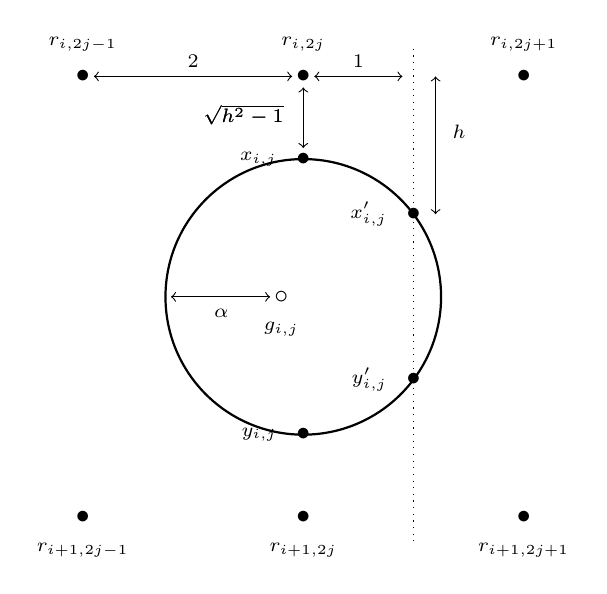
\begin{tikzpicture}[scale=7]

	
	\node[label=90:\scriptsize $r_{i,2j-1}$] at (0.1,0) {$\bullet$};
	\node[label=90:\scriptsize $r_{i,2j}$] at (0.5,0) {$\bullet$};
	\node[label=90:\scriptsize $r_{i,2j+1}$] at (0.9,0) {$\bullet$};
	
	\node[label=180:\scriptsize $\sqrt{h^2-1}$] at (0.5,-0.07) {};
	\node[label=180:\scriptsize $x_{i,j}$] at (0.5,-0.15) {$\bullet$};
	
	
	\node[label=180:\scriptsize $h$] at (0.83,-0.1) {};
	\node[label=180:\scriptsize $x_{i,j}'$] at (0.7,-0.25) {$\bullet$};
	
	\node[label=270:\scriptsize $g_{i,j}$] at (0.46,-0.4) {$\circ$};
	
	
	\node[label=180:\scriptsize $y_{i,j}$] at (0.5,-0.65) {$\bullet$};
	\node[label=180:\scriptsize $y_{i,j}'$] at (0.7,-0.55) {$\bullet$};
	
	
	\node[label=270:\scriptsize $r_{i+1,2j-1}$] at (0.1,-0.8) {$\bullet$};
	\node[label=270:\scriptsize $r_{i+1,2j}$] at (0.5,-0.8) {$\bullet$};
	\node[label=270:\scriptsize $r_{i+1,2j+1}$] at (0.9,-0.8) {$\bullet$};
	
	
	\node[label=180:\scriptsize $\sqrt{h^2-1}$] at (0.5,-0.07) {};
	
	
	\node[label=180:\scriptsize $\alpha$] at (0.4,-0.43) {};
	\node[label=90:\scriptsize $1$] at (0.6,-0.02) {};
	\node[label=90:\scriptsize $2$] at (0.3,-0.02) {};
	
	
	\draw[<->] (0.5,-0.13) -- (0.5,-0.02);
	\draw[<->] (0.26,-0.4) -- (0.44,-0.4);
	\draw[dotted,-] (0.7, 0.05) -- (0.7, -0.85);
	\draw[<->] (0.74, 0.0) -- (0.74, -0.25);
	\draw[<->] (0.68, 0.0) -- (0.52, 0.0);
	\draw[<->] (0.12, 0.0) -- (0.48, 0.0);
	\draw[black, thick] (0.5,-0.4) circle (0.25);
\end{tikzpicture}


\ifdefined\COMPLETE
\else
\end{document}
\fi
